\documentclass[10pt,a4paper,notitlepage,twocolumn]{report}
\usepackage{graphicx}
\usepackage{subfig}
\usepackage{multicol}
\usepackage{IEEEtrantools}
\usepackage{times}

\usepackage[margin=0.8in]{geometry}

\twocolumn \flushbottom \sloppy
\date{}

% The document begins
\title{Taster Project: Model-based 3D Single Hand Pose Estimation using Kinect}
\author{Andrew Chambers}
\begin{document}

\maketitle

\begin{abstract}

	This report details the implementation of a method described by Oikonomidis et 
	al~\cite{bmvc2011oikonom} for full 3D hand pose estimation given input from a 
	Kinect~\cite{kinect} RGB-D camera.  The method proposed is model-based, uses a 
	hand model composed of simple geometric primitives and optimises over 
	parameter space using a variant of Particle Swarm Optimisation.  The massively 
	parallel nature of modern GPUs is exploited to significantly improve the speed 
	of rendering and calculation of the objective function, and the result is a 
	system which can robustly infer full 3D hand pose at 10fps.

\end{abstract}

\section{Introduction}

Knowledge of hand pose from visual information is a process performed 
implicitely by humans, and is considered a fundamental component of human 
communication.  Hand pose inference is therefore an important problem in 
computer vision and while there have been great advances in the field in recent 
years, reliable and efficient estimation of hand pose is still an unsolved 
problem.  The applications of a robust system for infering hand pose from images 
are far reaching, and success in this area would provide the groundwork for sign 
language recogition, robot learning by example, or for gesture recognition and 
human computer interaction.

Difficulties are introduced by many factors, such as the high dimensionality of 
the problem or the articulate nature of the hand and its tendancy to 
self-occlude.   

Attempts to solve the problem can generally be seperated in to two groups; 
appearance-based solutions and model-based solutions, also known as 
discriminitive and generative solutions respectively.  

Appearance-based solutions use a large training dataset to learn a mapping from 
image features to a vector of hand pose parameters.  Differences between 
techniques comes down to different image features, and the choice of regression 
used for the mapping.  After the mapping is learnt, appearance-based solutions 
tend to be fast to infer pose, however since they only learn form what is given 
in the training dataset, suffer from inaccurate prediction when given a pose not 
present in the training data.

Model-based solutions rely on a parametric hand model which can be rendered 
given known intrinsic and extrinsic camera properties and hand pose parameters.  
Comparing the result of this rendering to image cues derived from an 
observation, we can calculate a measure of similarity between the observation 
and the estimation.  By searching parameter space and maximising this 
similarity, we find a hand pose which most closely matches that of the pose in 
the observed image.  Model-based solutions can accurately infer any hand pose, 
given that it is possible to search all of the hand pose parameter space.  They 
do, however rely heavily on initialisation since it is intractable to search the 
whole of parameter space, and since rendering and calculation of the similarity 
function is costly, can be slow to converge on a solution.

This report gives details of an implementation of a method for hand pose 
estimation proposed by Oikonomidis et al~\cite{bmvc2011oikonom}.  This method is 
model-based, uses a Kinect RGB-D image cues, a composite hand model, and 
particle swarm optimisation to search parameter space.  The massively parallel 
architecture of modern GPUs is exploited to significantly speed up the parameter 
search process.

\section{Related Work}
Erol et al~\cite{erol2007vision} present a thorough review of hand pose 
estimation techniques, and based how complete the pose estimation result is, are 
described as either partial or full estimation techniques.  Full pose estimation 
techniques are further separated into either model-based, or appearance-based 
which elsewhere in the literature are more generally known as generative and 
discriminitive methods respectively.  

Model-based methods require a deformable, articulated hand model which is 
rendered in order to generate an image similar to image cues extracted from an 
observation.  An objective function allows optimisation over parameter space.  
These methods differ in the hand model used, the image cues extracted, and then 
by parameter optimisation. 

Gorce and Paragios~\cite{de2008model} present a method which uses a realistic 
triangular mesh hand model and having chosen a differentiable objective 
function, use gradient descent to optimise over parameter space.  The system 
appears to work well, however evaluation is only done on a small test sequence 
with limted hand movement and finger articulations.  Oikonomidis et 
al~\cite{oikonomidis2011markerless} present a system which uses a quadric based 
hand model, a multicamera system and distance image cues, and Particle Swarm 
Optimisation (PSO) to find hand pose parameters.  Since PSO is used, the 
optimisation is trivially paralellisable, and the system is capable of near real 
time speed.  This work has been extended to hand interactions with static 
objects~\cite{oikonomidis2011}, and also allowing full pose estimation of two 
hands~\cite{oikonomidis2012}.  The method implemented in this report is based on 
a further extension of this work which relies on a Microsoft 
Kinect~\cite{kinect} sensor for observation~\cite{bmvc2011oikonom}.

Appearance-based methods learn a mapping from a set of image features extracted 
from an observation, to a set of hand pose configurations.  These methods vary 
in the image features used, the method employed to learn the mapping, and the 
scale of the training set used.  

Athitsos et al~\cite{athitsos2003estimating} produce a set of synthetic images 
of 26 hand shapes viewed from 88 different viewpoints.  Each image is then 
replicated with 48 uniform in-plane rotations.  This image database is then used 
to match a pose to an observation image in a two stage process.  The first stage 
quickly removes highly unlikely poses, and the second phase more thoroughly 
matches the observation to a pose.  This approach suffers from only using a 
small set of example poses.  De Campos~\cite{de2006regression} presents a 
regression-based method for hand pose estimation which uses shape context 
descriptors and multiple views to improve accuracy, developing on earlier work 
proposed by Agarwal and Triggs~\cite{agarwal2006recovering}.  Romero et 
al~\cite{romero2009monocular} use HOG features, a synthetic image dataset of 
$10^5$ images, and a nearest neighbour search in HOG space.  Since they are 
searching for hand pose in a temporal image sequence, they enforce temporal 
continuity during the search by limiting the search space which improves 
accuracy.

\section{Method}

The method implemented, as with many model based solutions is split in to three 
stages.  Firstly the hand region is segmented from the observation, secondly a 
hand pose is rendered, and thirdly this is compared to the observation.  This is 
complicated by the exploitation of the highly parallel nature of the second and 
third stages.  By rendering many hand poses at the same time, and also 
calculating the similarity of each rendering to the observation in parallel, we 
can speed up the parameter search significantly.  Stage one is discussed in 
section~\ref{subsec:segmentation}, stage two in section~\ref{subsec:hand_model} 
and stage three in section~\ref{subsec:pose_selection}.

	\subsection{Segmentation of the hand}
	\label{subsec:segmentation}

	Segmentation is the process of separating a subject in an image from the 
	background.  In the case of hand pose estimation, this means producing an 
	image mask whereby a 1 corresponds to a pixel which is known to belong to the 
	hand, and a 0 otherwise.  The method implemented uses skin colour and depth 
	from the Kinect sensor to determine the pixel labelling.  
  
	Pixels from the RGB sensor are classified according to the method given
	in~\cite{argyros2004real-timetracking}.  This uses a non-parametric Bayes
	classifier trained using the dataset produced by Jones et
	al~\cite{jones2002statisticalcolor} to assign a probability to each pixel in
	the image corresponding to the likelihood that the pixel is skin.  With this
	``Probability image'', hysteresis thresholding is then used to produce a
	binary image in which pixels are either labelled as skin or not skin.  This
	process involves marking pixels as skin if their probability is greater than
	$t_1$, and then scanning recursively outwards from these ``Seed'' pixels, and
	marking others as skin if their probability is higher than $t_2$.  The Kinect
	depth image is also used to aid segmentation.  Firstly pixels which are of
	depth greater than $t_D$ are ignored.  This completely elliminates unwated
	background noise.  Pixels are labelled as skin if the depth of that pixel is
	not more than $t_d$ from any skin pixels in the previous frame.  This helps
	to reduce the effects of noise in the RGB image.  Finally the largest
	connected component is selected from this binary image, dilated, and chosen
	as the hand region.

	\subsection{The hand model}
	\label{subsec:hand_model}

	The model used for rendering is a composite model made of transformed
	cylinders and spheres.  This model is chosen due to the simplicity with which
	it can be articulated, and the speed at which it can be rendered.  Since each
	primitive is an instance of either a sphere or a cylinder, hardware
	instancing is used.  Hardware instancing is a technique employed by modern
	GPUs which greatly improves rendering speed by exploiting the fact that each
	primitive is the same shape with a different transformation applied to it.
	This greatly reduces the amount of vertex data sent across the PCI bus to the
	GPU, and thus improves rendering speed.  An image of the hand model is given
	in figure~\ref{fig:hand_model}.

	\begin{figure}
		\centering
		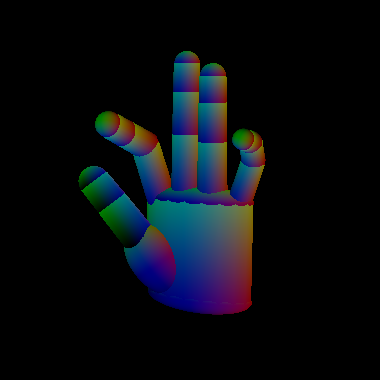
\includegraphics[width=0.8\linewidth]{images/hand_render}
		\caption{Image of a rendering of the deformable hand model}
		\label{fig:hand_model}
	\end{figure}

	The aim of rendering is to produce an image which looks identical to the
	observation.  Since our observation is a binary skin image and a Kinect depth
	image, we render each fragment as a greyscale value which is the interpolated
	world space depth value passed from the vertex shader.

	\subsection{Pose selection}
	\label{subsec:pose_selection}

	In order to estimate pose parameters accurately, a search over parameter space 
	is required.  

	We first formally define our observation and hypothesis.  Our segemented hand
	image, $o_s$ is a binary mask which is set to 1 if the pixel in our obseration
	belongs to the hand, and 0 otherwise.  The observed depth image, $o_d$ is a
	raw image captured from the Kinect sensor, which gives depth values from the
	camera in millimeters.  Our rendering, $r_d(h, C)$ gives the depth in
	world units of the rendered hypothesis $h$ from the camera $C$.  We produce a
	binary map $r_m(h, C)$ in which a pixel is set as 1 if the respective depths
	of a pixel in $r_d$ and $o_d$ differ by less than a predetermined value,
	$d_m$ or if $o_d$ is 0, and set to 0 otherwise.  If $o_d$ has a value of 0,
	this means the observation is too close to the camera, and we assume that in
	this case the pixel corresponds to the hand. Given these
	definitions, we define the objective function $E(h, O)$.
  
\begin{equation}
	E(h, O) = D(O, h, C) + \lambda_{k} \cdot kc(h) \end{equation}

$D(O, h, C)$ is a distance measure which gives the similarity of the observation 
to the hypothesis.

\begin{equation}
	\label{eq:d}
	\begin{IEEEeqnarraybox}{rCl}
	D(O, h, C) & = & \frac{ \sum min(|o_{d} - r_{d} | , d_{M}) }
										{ \sum (o_{s} \vee r_{m}) + \epsilon } \nonumber\\
	&& +\: \lambda \left ( 1 - \frac { 2 \sum (o_s \wedge r_m)}
														{\sum (o_s \wedge r_m) + \sum (o_s \vee r_m)} \right 
														)
	\end{IEEEeqnarraybox}
\end{equation}

The first term is a measure of the absolute difference between the clamped depth 
of the observation and the rendered hypothesis.  We clamp depths to a 
predetermined value $d_M$ as inaccurate hand segmentation may lead to a 
reasonable hypothesis being penalised.  The second term penalises discrepencies 
between the skin coloured pixels in the observation and rendering.

The second term of $E(h, O)$, $kc(h)$  penalises kinectically implausible 
hypotheses and is defined as $kc(h) = \sum_{p \in Q} - min(\phi(p, h), 0)$.  $Q$ 
denotes the three pairs of adjacent fingers (Excluding the thumb), and $\phi$ is 
the difference in radians of the adduction-abduction angles of those fingers in 
hypothesis $h$.  During the implementation, values of $d_m$, $d_M$ were set to 
$1cm$ and $4cm$ respectively, while $\lambda$ and $\lambda_k$ were 20 and 10 
respectively, as given in the original paper~\cite{bmvc2011oikonom}.

		\subsubsection{Particle Swarm Optimisation}

	The parameter search method chosen for this implementation is Particle Swarm
Optimisation~\cite{kennedy1995particle}.  Particle Swarm Optimisation is a
nature inspired evolutionary optimisation algorithm in which a swarm of
``Particles'' exist in parameter space. The swarm exists for a set number of
generations, and each particle moves according to information about the value of
the objective function discovered itself and by other particles in the swarm.
Finally, the optimum foud by the swarm is the best value of the objective
function found by any particle over all generations.

	Each particle stores its current position $x_k$ and its current velocity 
	$v_k$.  Also stored is $P_k$, a record of its best position, or the position 
	at which it achieved the lowest value from the objective function up to 
	generation $k$.  The position $G_k$, the current global optimum or the best 
	position that any particle in the swarm has achieved up to generation $k$ is 
	broadcast to the entire swarm.  Each generation, the position and velocity of 
	each particle is updated accordording to equations~\ref{eq:posupdate} 
	and~\ref{eq:velupdate}.

\begin{equation}
	\label{eq:posupdate}
	x_{k+1} = x_k + v_{k+1}
\end{equation}

\begin{equation}
	\label{eq:velupdate}
	v_{k+1} = w(v_k + c_1r_1(P_k - x_k) + c_2r_2(G_k - x_k)), \end{equation}

where $w$ is a constant, $r_1$ and $r_2$ are uniformly sampled random numbers
between 0 and 1, and $c_1$ and $c_2$ are termed the cognitive and social
components respectively as defined by .  As suggested, $c_1 = 2.8$, $c_2 = 1.3$,
and $w = 2 / \left | 2 - \psi - \sqrt{\psi^2 - 4 \psi} \right |$ with $\psi =
c_1 + c_2$.  After $k$ generations, $G_k$, the global best position is the
result of the optimisation.

For this application, the position of each particle in space represents the
value of each of the pose parameters of the hypothesis, and thus the parameters
with which to render the hand model and evaluate the objective function.  Each
particle represents a different hand pose, and the best position over all $k$
generations, $h_{best}$ is chosen as the best estimate of hand pose for the 
observation.

Since this system operates on a temporal image sequence, and since the position
and articulation of the hand will differ only a small amount from the previous 
frame,
perturbations of $h_{best}$ from frame $F_t$ are used as initial particle
positions for the next frame $F_{t+1}$.  This ensures that the parameter search
for the next frame is initialised closely to the expected solution.  The
deviation of other particles in the swarm from $h_{best}$ is determined
experimentally and depends on the speed of hand motion in the image sequence and
the framerate.

\subsection{GPU Acceleration}

Several components of this implementation are parallelisable, and since modern
GPUs are programmable, the implementation follows the framework given
in~\cite{kyriazis2011} to make better use of available hardware and improve
performance.

\subsubsection{Tiled rendering}

Rendering can be a costly operation, but the hand model we are rendering is
simple and requires little GPU power to be drawn.  Because of this, a single
draw call will not be utilising the full capacity of a modern GPU, and we are
wasting resources.  To improve upon this, we render many hand poses
simultaneously in a large tiled rendering.  The size of the rendering
corresponds to the number of particles in the swarm, meaning a single rendering 
is all that is required for each swarm generation.  This is an optimum use of
GPU resources, since the position of particles in generation $k+1$ is
dependent on the objective function result of particles in generation $k$.

\subsubsection{Objective function evaluation}

In recent years, GPUs have evolved to perform not just graphics rendering, but
general computation as well, allowing the exploitation of their
parallel architecture.  OpenCL~\cite{opencl1.2spec}, a platform which allows us
to produce programs to execute on a GPU, is used to reduce the summations within
the distance function $D(O, h, C)$ given in equation~\ref{eq:d}.  Since the
large tiled rendering is written to memory on the graphics card, and we evaluate
the objective function on the GPU as well, only the result of the objective 
function is copied across the PCI bus.

\section{Results}

Work is still ongoing on quantitative evaluation of the implemented system,
however preliminary qualitative results are given.

\subsection{Qualitative results}

Figure~\ref{fig:results1} shows several images captured during the tracking.

\section{Conclusion}

This report gives details of the implementation of a system for full 3D hand
pose estimation.  The system implemented is based on a paper by Oikonomidis et
al~\ref{bmvc2011oikonom}.  The implemented system functions well, and is capable
of tracking a single hand at near real-time speeds (10fps).  The tracking is
fairly accurate for 3D global position and finger articulation, but struggles
with fast movements and global orientation changes.  Skin segmentation and the
poor quality of the Kinect RGB camera contribute to these problems, but further
work is being done to improve segmentation and overcome these issues.  Further
tuning of Particle Swarm parameters may lead to better finger articulation
estimation. 

% Now print the bibliography
\bibliographystyle{plain}
\bibliography{report}

\end{document}
